
\chapter{Detailed Analysis and Comparison of Results}
\label{cha:conclusions_future_directions}
In this chapter we present the benchmark results on different tecnologies and strategies on the two chose algorithms previously mentioned in previous chapter, as detailed in the preceding chapters. Our investigation spanned various strategies and implementations, culminating in a nuanced understanding of the relative performance and characteristics of different approaches across .NET, Java, and other programming environments. Here, we consolidate these findings, reflecting on their broader implications within the field of asynchronous programming. Furthermore, we outline potential avenues for future research that emerge from our study, paving the way for continued exploration and innovation in this domain.


\section{.NET Benchmarking}
\label{sec:dotnet_implementation}

In this subsection, we focus on the benchmark using different strategies in .NET programming environment.


\subsection{Find the biggest word algorithm results}
\label{subsubsec:biggest_word_results_cs}

For the find the biggest word algorithm, used i .NET implementations are the following strategies:

\begin{itemize}
    \item \textbf{Baseline}: This strategy serves as the basic approach for finding the biggest word and acts as a baseline for comparison.
    \item \textbf{Asynchronous Baseline }: This strategy uses a single asynchronous task to find the biggest word.
    \item \textbf{Parallel }: An approach that makes the use of parallelization.
    \item \textbf{AsyncEnumerable}: This approach uses asynchronous programming with enumerable collections.
    \item \textbf{RxNet }: This strategy uses the Reactive Extensions (Rx) library with asynchronous file reading operations.
\end{itemize}


In the following graphic, we have the results in seconds for each strategy:

\begin{figure}[H]
    \centering
    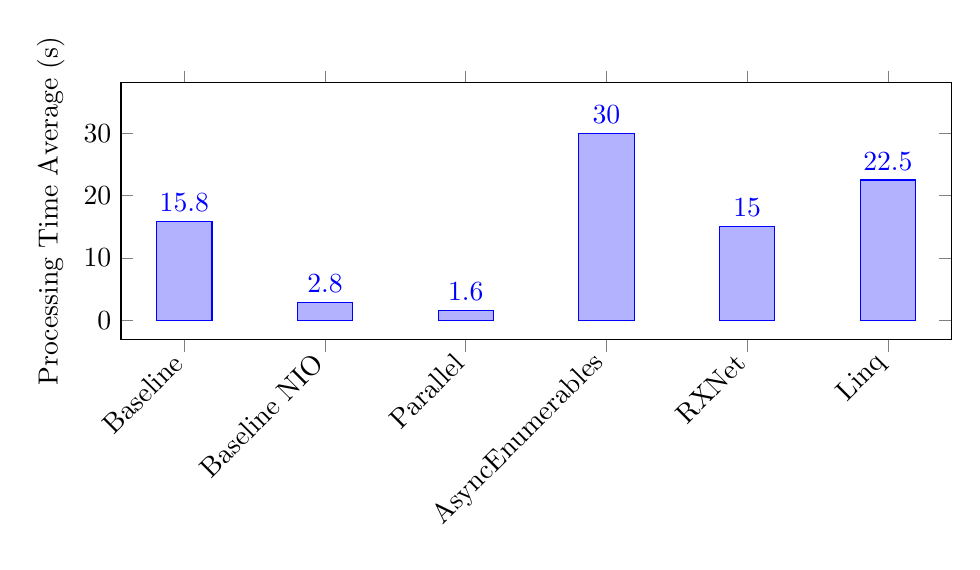
\begin{tikzpicture}
    \begin{axis}[
        ybar=2*\pgflinewidth,
        width=1.0\textwidth,
        height=0.4\textwidth,
        bar width=20pt,
        enlargelimits=0.09,
        legend style={at={(0.5,-0.2)}, anchor=north, legend columns=-1},
        ylabel={Processing Time Average (s)},
        symbolic x coords={Baseline, Baseline NIO, Parallel, AsyncEnumerables, RXNet, Linq},
        xtick=data,
        xticklabel style={rotate=45, anchor=east},
        nodes near coords,
        nodes near coords align={vertical},
        ymin=0, ymax=35,
        ]
    \addplot coordinates {(Baseline, 15.8) (Baseline NIO, 2.8) (Parallel, 1.6) (AsyncEnumerables, 30) (RXNet, 15) (Linq, 22.5)};
    \end{axis}
    \end{tikzpicture}
    \caption{Processing times for different strategies for "Find the biggest word".}
    \label{fig:biggest_word_results_cs_2}
\end{figure}


From these results, it is apparent that the asynchronous baseline approach has an advantage over its blocking counterpart. However, it is also evident that the parallel solution holds an advantage over its pipeline competitors.

Taking into account the pipeline technologies, we can see that the overall performance is worse compared to strategies that do not use pipelines. In this context, RxNet demonstrates a performance advantage over both Linq and AsyncEnumerables strategies. However, it was expected that, since Linq uses a blocking IO source, it would perform worse than AsyncEnumerables, but that does not occur. This may imply that for this particular algorithm, the AsyncEnumerable strategy incurs a higher overhead than intended.

\clearpage


\subsection{Group Word Results}
\label{subsubsec:group_word_processing_times_cs}

In this subsection, we concentrate on the task of grouping words from a file using different strategies. The strategies that we evaluate here include:

\begin{itemize}
    \item \textbf{Baseline}: This strategy serves as the basic approach for word grouping and acts as a baseline for comparison.
    \item \textbf{Linq}: Like in the find word algorithm, this strategy uses Language Integrated Query (LINQ) in a synchronous manner.
    \item \textbf{AsyncEnumerable}: This strategy uses .NET async enumerables to process the asynchronous data .
    \item \textbf{RxNet}: Here, the Reactive Extensions (Rx) library is used to handle data sequences asynchronously and event-based.
\end{itemize}


\begin{figure}[H]
    \raggedright
    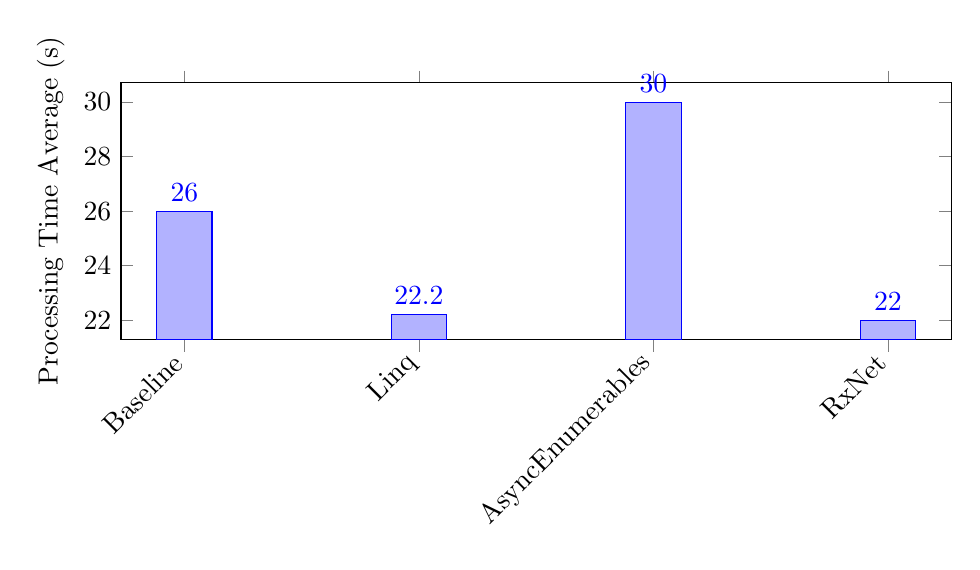
\begin{tikzpicture}
    \begin{axis}[
        ybar=2*\pgflinewidth,
        width=1.0\textwidth,
        height=0.4\textwidth,
        bar width=20pt,
        enlargelimits=0.09,
        legend style={at={(0.5,-0.2)}, anchor=north, legend columns=-1},
        ylabel={Processing Time Average (s)},
        symbolic x coords={Baseline, Linq, AsyncEnumerables, RxNet},
        xtick=data,
        xticklabel style={rotate=45,anchor=east},
        nodes near coords,
        nodes near coords align={vertical},
        ]
    \addplot coordinates {(Baseline, 26.0) (Linq, 22.2) (AsyncEnumerables, 30) (RxNet, 22.0)};
    \end{axis}
    \end{tikzpicture}
    \caption{Processing times for different strategies for "Count Words".}
    \label{fig:group_word_processing_times_cs}
\end{figure}

The baseline strategy serves as a fundamental approach to word grouping and establishes a standard for performance comparison. While straightforward, it does not leverage the advanced features of other approaches, resulting in a moderate processing time. In comparison, the Linq strategy, utilizing Language Integrated Query in a synchronous manner, shows an improvement in performance over the baseline. This suggests that the streamlined querying capabilities of LINQ, despite being synchronous, can efficiently handle the algorithm's requirements.

On the other hand, the AsyncEnumerable approach, which uses .NET async enumerables to process asynchronous data, exhibits a longer processing time in this context. This indicates that while async enumerables are beneficial for certain applications, their performance in memory-intensive tasks like "Group Words," which heavily relies on dictionaries, might not be optimal.

Furthermore, the RxNet implementation, employing the Reactive Extensions library to handle data sequences asynchronously and event-based, also demonstrates competitive performance. This underscores the potential of RxNet in efficiently managing asynchronous data flows, especially in scenarios where the processing time is crucial.

Overall, while pipeline libraries tend to outperform the baseline approach in memory-intensive algorithms like "Group Words," the choice between blocking and non-blocking IO operations becomes less significant. This is primarily because the overhead from memory-intensive operations tends to overshadow any potential performance gains from using non-blocking IO operations. The results indicate that the optimal strategy for such algorithms would depend more on how they handle memory-intensive operations rather than the differences in IO operation types.
\clearpage

\section{Java/Kotlin Benchmarking}
\label{sec:java_implementation}

In this section, we explore and assess diverse strategies applied in Java and Kotlin to process files, and we scrutinize their performances solving the "Find Word" an "Group Word algorithms"


\subsection{Biggest Word Results}
\label{subsubsec:biggest_word_results}

The strategies used in JAVA are:

\begin{itemize}
    \item \textbf{Baseline}: This strategy illustrates a basic non-blocking I/O operation, serving as a comparison baseline.
    \item \textbf{Flux}: These strategies leverage the Reactor Flux model from Java's Project Reactor library. The former follows a standard non-concurrent processing model, while the latter introduces parallelization for improved performance.
    \item \textbf{RXJava}: This strategy employ the RXJava library. They replace the Reactor Flux with Observables, with the distinction being made between non-concurrent and concurrent processing.
    \item \textbf{Streams and parallelization}: Implementation of three strategies that use Java's Streams API and explore handling of blocking operations under three different conditions: standard usage, raw multithreading using threadpools and using parallel method in the streams API.
    
\end{itemize}


In the following graphic, we have the results in seconds for each strategy:

    \begin{figure}[H]
        \raggedright
        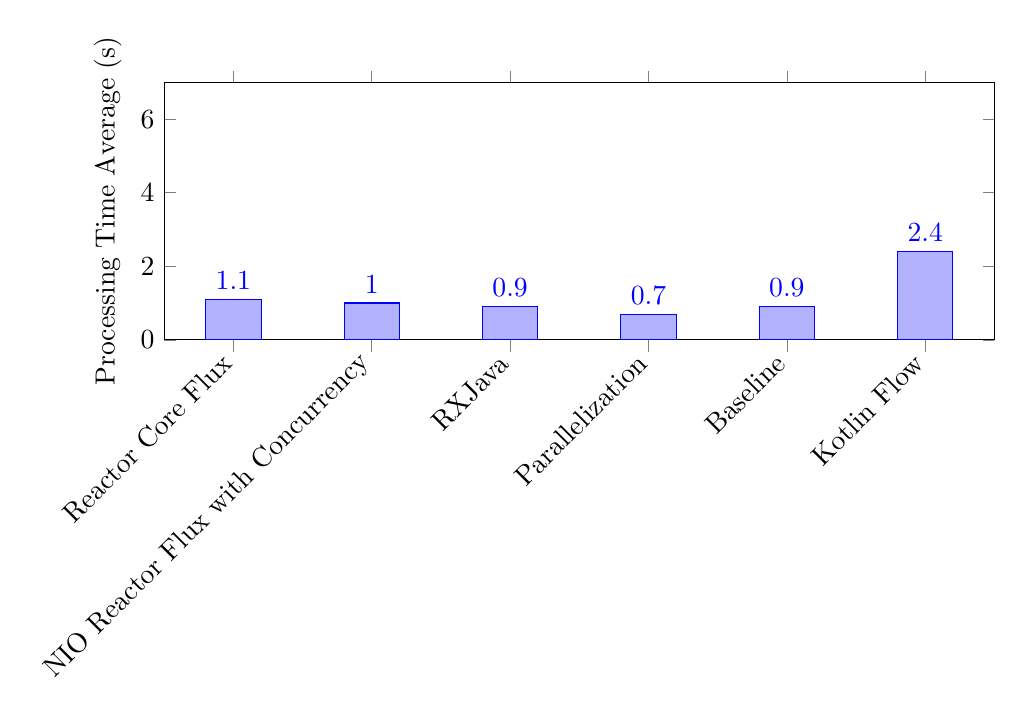
\begin{tikzpicture}
        \begin{axis}[
            ybar=2*\pgflinewidth,
            width=1.0\textwidth,
            height=0.4\textwidth,
            bar width=20pt,
            legend style={at={(0.5,-0.2)}, anchor=north, legend columns=-1},
            ylabel={Processing Time Average (s)},
            symbolic x coords={Reactor Core Flux, NIO Reactor Flux with Concurrency, RXJava, Parallelization, Baseline, Kotlin Flow},
            xtick=data,
            xticklabel style={rotate=45,anchor=east},
            nodes near coords,
            nodes near coords align={vertical},
            ymin=0, ymax=7,
            ]
        \addplot coordinates {(Baseline, 0.9) (Reactor Core Flux, 1.1) (NIO Reactor Flux with Concurrency, 1.0) (RXJava, 0.9) (Parallelization, 0.7) (Kotlin Flow, 2.4) };
        \end{axis}
        \end{tikzpicture}
        \caption{Processing times for different Java/Kotlin strategies for "Biggest Word".}
        \label{fig:biggest_word_processing_times}
    \end{figure}
    

    For the "Biggest Word" results, the strategies exhibit varied performance levels. The Baseline strategy, illustrating basic non-blocking I/O operations, provides a solid foundation for comparison and demonstrates a competent processing time. Flux strategies, both Reactor Core Flux and its concurrent variant, leverage the Project Reactor library to enhance processing, showing slight variations in efficiency. The RXJava strategy, utilizing the RXJava library, aligns closely with the baseline in terms of performance. A notable distinction is seen in the strategies employing parallelization, particularly those using Java's Streams API, which show the most efficient processing times. This underscores the advantage of parallel processing in optimizing performance.

    \clearpage

    \subsection{Group Word Results}
    \label{subsubsec:group_word_results}
    
   The strategies discussed here include:

    \begin{itemize}
        \item \textbf{Baseline}: This strategy serves as a baseline for comparison. It illustrates a basic non-blocking I/O operation without the use of any high-level constructs like Reactor Flux or Observable.
        \item \textbf{RXJava}: This strategy employs the RXJava library, popular for building asynchronous and event-driven applications.
        \item \textbf{Reactor Core Flux}: This strategy leverages the Reactor Flux model available in Java's Project Reactor library, providing an efficient approach to handling asynchronous data sequences.
        \item \textbf{Parallel}: This strategy uses Java's Streams API and explores handling of blocking operations with the help of threadpools.
        \item \textbf{Flow (Kotlin)}: This strategy utilizes Kotlin's Coroutines and Flow API, which are particularly well-suited for handling multiple values that are emitted sequentially.
    \end{itemize}

    In the following table and graphic, we have the results in seconds for each strategy:

    \begin{figure}[H]
        \centering
        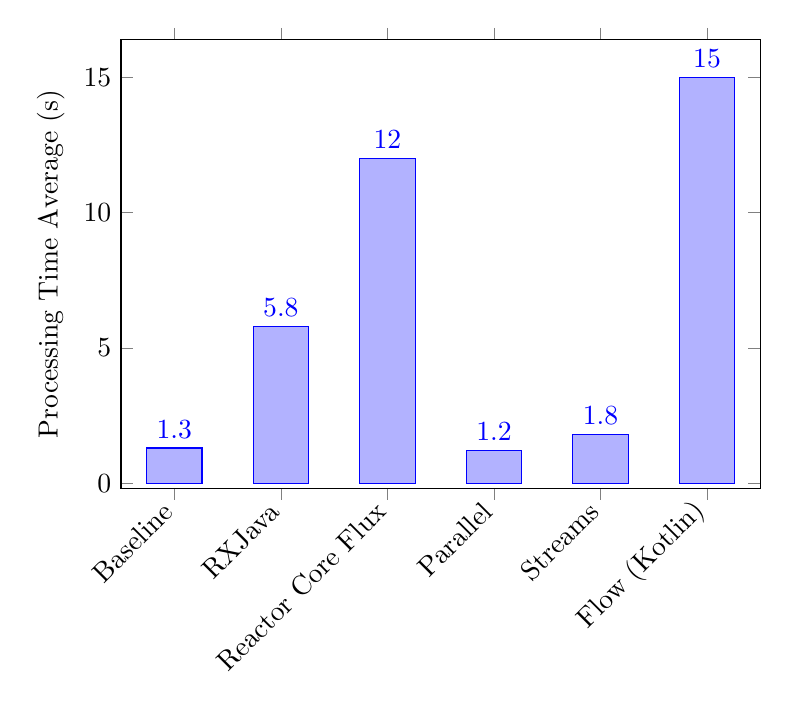
\begin{tikzpicture}
        \begin{axis}[
            ybar=2*\pgflinewidth,
            width=0.8\textwidth,
            height=0.6\textwidth,
            bar width=20pt,
            legend style={at={(0.5,-0.2)}, anchor=north, legend columns=-1},
            ylabel={Processing Time Average (s)},
            symbolic x coords={Baseline, RXJava, Reactor Core Flux, Parallel, Streams, Flow (Kotlin)},
            xtick=data,
            xticklabel style={rotate=45,anchor=east},
            nodes near coords,
            nodes near coords align={vertical},
            ]
            \addplot coordinates { (Baseline, 1.3) (RXJava, 5.8) (Reactor Core Flux, 12.0) (Parallel, 1.2) (Streams, 1.8) (Flow (Kotlin), 15.0)};
        \end{axis}
        \end{tikzpicture}
        \caption{Processing times for different Java/Kotlin strategies for "Group Words".}
        \label{fig:processing_times}
    \end{figure}
    

    \clearpage
    
    On "Group Word" benchmark results, the strategies again present a range of performances. The Baseline strategy, as before, sets a standard for comparison, showing moderate efficiency. RXJava, known for its asynchronous and event-driven capabilities, demonstrates a longer processing time in this context, indicating potential overheads in handling complex data sequences. Reactor Core Flux, while efficient in handling asynchronous sequences, shows a significant processing time, possibly due to the complexity of the Group Word algorithm. Strategies involving parallel processing, whether through direct use of threadpools or the Streams API, exhibit improved efficiency, highlighting the benefits of parallelism in handling computationally and memory intensive tasks. Notably, Kotlin's Flow API, designed for handling sequential emissions in a coroutine-based environment, shows a longer processing time, which could reflect the overheads associated with coroutine management in complex data processing scenarios.


    Overall to JAVA, these results illustrate the trade-offs between different programming paradigms and libraries in Java and Kotlin. While some strategies excel in simple tasks, others are more suited to complex algorithms, indicating the importance of choosing the right approach based on the specific requirements of the algorithm and the nature of the data being processed.


\section{JavaScript Benchmarking}
\label{sec:js_implementation}


\subsection{Finding the Biggest Word}
\label{subsec:biggest_word_js}

Here, we investigate the following three strategies:

\begin{itemize}
    \item \textbf{Baseline}: This strategy serves as the basic JavaScript approach for finding the biggest word, acting as a baseline for comparison.
    \item \textbf{Stream}: This strategy uses JavaScript streams, which provide a way to handle reading/writing files, network communications, or any kind of end-to-end information exchange in an efficient manner.
    \item \textbf{RxJS}: This strategy leverages the Reactive Extensions for JavaScript (RxJS) library, which offers a set of methods for dealing with asynchronous data sequences in an effective way.
\end{itemize}


In the following graphic, we have the results in seconds for each strategy:


\begin{figure}[H]
    \raggedright
    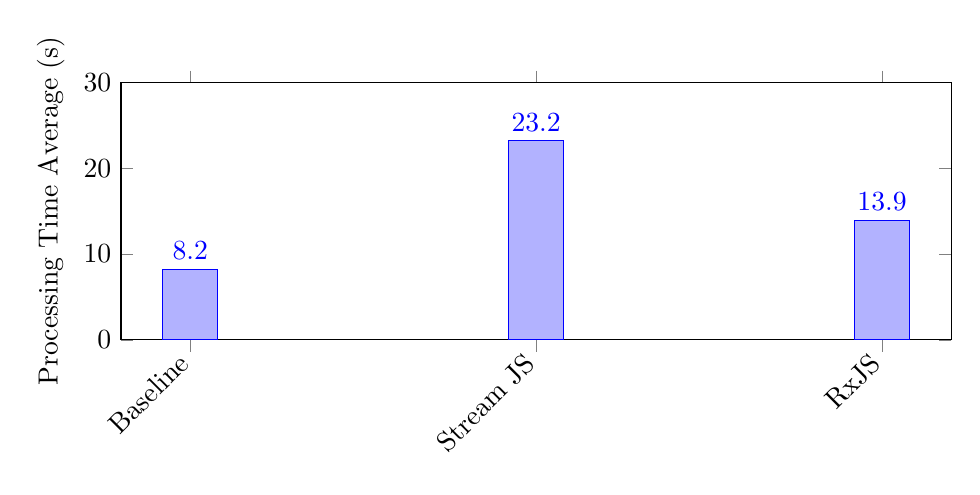
\begin{tikzpicture}
    \begin{axis}[
        ybar=2*\pgflinewidth,
        width=1.0\textwidth,
        height=0.4\textwidth,
        bar width=20pt,
        legend style={at={(0.5,-0.2)}, anchor=north, legend columns=-1},
        ylabel={Processing Time Average (s)},
        symbolic x coords={Baseline, Stream JS, RxJS},
        xtick=data,
        xticklabel style={rotate=45,anchor=east},
        nodes near coords,
        nodes near coords align={vertical},
        ymin=0, ymax=30,
        ]
    \addplot coordinates {(Baseline, 8.2) (Stream JS, 23.2) (RxJS, 13.9)};
    \end{axis}
    \end{tikzpicture}
    \caption{Processing times for different JavaScript strategies for "Biggest Word" Graphic}
    \label{fig:biggest_word_processing_times_js}
\end{figure}

As we can see in this javascript implementation, the performance for find biggest word algorithm of the baseline behaves as expected, having the best performance among its alternatives. On the other side, the algorithm implemented using RXJS library behaves slightly better than the alternative that makes use of JS streams API.


\clearpage



\subsection{Grouping Words}
\label{subsec:grouping_words_js}

In this subsection, we evaluate the following strategies for grouping words:

\begin{itemize}
    \item \textbf{Baseline}: This strategy serves as the basic JavaScript approach for grouping words, acting as a baseline for comparison.
    \item \textbf{Stream JS}: This strategy uses JavaScript streams, which provide a way to handle reading/writing files, network communications, or any kind of end-to-end information exchange in an efficient manner.
    \item \textbf{RxJS}: This strategy leverages the Reactive Extensions for JavaScript (RxJS) library, which offers a set of methods for dealing with asynchronous data sequences in an effective way.
\end{itemize}

In the following graphic, we present the results in seconds for each strategy:


\begin{figure}[H]
    \centering
    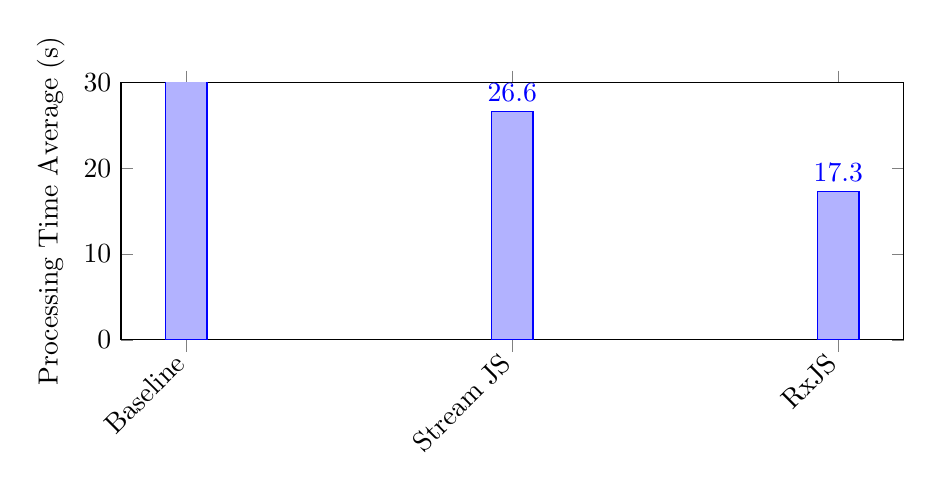
\begin{tikzpicture}
    \begin{axis}[
        ybar=2*\pgflinewidth,
        width=0.95\textwidth,
        height=0.4\textwidth,
        bar width=15pt, % Reduced bar width
        legend style={at={(0.5,-0.2)}, anchor=north, legend columns=-1},
        ylabel={Processing Time Average (s)},
        symbolic x coords={Baseline, Stream JS, RxJS},
        xtick=data,
        xticklabel style={rotate=45, anchor=east},
        nodes near coords,
        nodes near coords align={vertical},
        ymin=0, ymax=30,
        ]
    \addplot coordinates {(Baseline, 30.1) (Stream JS, 26.6) (RxJS, 17.3)};
    \end{axis}
    \end{tikzpicture}
    \caption{Processing times for different JavaScript strategies for "Grouping Words" Graphic}
    \label{fig:grouping_words_processing_times_js}
\end{figure}



In this case, the performance of the algorithms change radically from what we saw in the "Find the biggest word" algorithm. In this case, the baseline haves the worst performance among the three strategies, while the RxStrategy haves the best. 
One explanation for these results is that the pipeline instructions of the pipeline instructions are optimized while the baseline is not. 